\section{Calculation of Complex Abundance}

All protein data quantified the abundance of individual proteins per cell.
However, this work requires estimates on the abundance of individual protein
\textit{complexes}, rather than the copy number of individual proteins. In our
analysis of the protein copy number data, it became clear that the reported copy
numbers do not always align with those based on reported stiochometry. As one
example of this, the F-O subunit of ATP synthase consists of three protein
subunits with a stiochometry of [AtpB][AtpF]$_2$[AtpE]$_{10}$ (also referred to
as subunits a, b, and c, respectively). In the experimental data of
\cite{schmidt2016}, the values deviate from this quite substantially, with
approximately 1000 AtpB, 9000 AtpF, and 300 AtpE reported per cell (minimal
media + glucose growth condition).  This highlights the technical challenges
that still remain in our ability to quantify cellular composition, particularly
for membrane-bound proteins like the ATP synthase complex considered here.  In
this section, we outline the approach we used to annotate proteins as part of
each macromolecular complex and how we used averaging across the individual
protein measurements to estimate an absolute complex abundances per cell.

Protein complexes, and proteins individually, often have a variety of names,
both longform and shorthand. As individual proteins can have a variety of
different synonyms, we sought to ensure that each protein annotated in the
data sets used the same synonym. To do use, we relied heavily on the EcoCyc
Genomic Database \citep{keseler2017}.  Each protein in available data sets
included an annotation of one of the gene name synonyms as well as an
accession ID -- either a UniProt or Blattner "b-number". We programmatically
matched up individual accession IDs between the proteins in different data sets.
In cases where accession IDs matched but the gene names were different, we
manually verified that the gene product was the same between the datasets and
chose a single synonym.  All code used  in the data cleaning and unification
procedures can be found on the associated
\href{https://github.com/rpgroup-pboc/growth_limits}[GitHub repository]
(DOI:XXX) associated with this paper as well as on the associated
\href{https://rpgroup.caltech.edu/growth_limits}{paper website}.

With each protein conforming to a single identification
scheme, we then needed to identify the molecular complexes each protein was a
member of. Additionally, we needed to identify how many copies of each protein
were present in each complex (i.e. the subunit copy number) and compute the
estimated abundance complex that accounted for fluctuations in subunit
stoichiometry. To map proteins to complexes, we accessed the
EcoCyc \textit{E. coli} database \cite{keseler2017} using PathwayTools version
23.0 \cite{karp2019}. With a license for PathWay Tools, we
mapped each unique protein to its annotated complexes via the
BioCyc Python package. As we mapped each protein with \textit{all} of its
complex annotations, there was redundancy in the dataset. For example, ribosomal
protein L20 (RplT) is annotated to be a component of the 50S ribosome (EcoCyc
complex \texttt{CPLX-03962}) as well as a component of the mature 70S ribosome
(EcoCyc complex \texttt{CPLX-03964}).

In addition to the annotated complex, we collected information on the
stoichiometry of each macromolecular complex. For a complex with $N_\text{subunits}$ protein species,
for each protein subunit $i$ we first calculate the number of complexes that
\textit{could} be formed given the measured protein copy numbers per cell,
\begin{equation}
    N_\text{complex}(\text{subunit i}) = \frac{P_\text{subunit i}^\text{(measured)}}{m_\text{subunit i}}.
    \label{eq:subunit_max}
\end{equation}
Here, $P_\text{subunit i}^\text{(measured)}$ refers to the measured protein copy number of species $i$,
and $m$ refers to the number of monomers present for that protein in the complex. For example, the 70S mature ribosome complex has 55 protein components, all of
which are present in a single copy except L4 (RplL), which is present in 4
copies ($m$ = 4). For each ribosomal protein, we then calculate the  maximum number of
complexes that could be formed using \EQ{subunit_max}. This example, along with
example from 5 other macromolecular complexes, can be seen in
\FIG{complex_counting}.

It is important to note that measurement noise, efficiency of protein
extraction, and differences in protein stability will mean that the precise value of each
calculation will be different for each component of a given complex. Thus, to
report the total complex abundance, we use the arithmetic mean of
across all subunits in the complex,
\begin{equation}
   \langle N_\text{complex} \rangle = \frac{1}{N_\text{subunits}}\sum\limits_i^{N_\text{subunits}} \frac{P_{i}^\text{(measured)}}{m_\text{subunit i}}.
   \label{eq:complex_count}
\end{equation}
in \FIG{complex_counting}, we show this mean value as a grey line for a variety
of different complexes. Additionally, we have built an interactive figure
accessible on the \href{https://www.rpgroup.caltech.edu/growth_limits}{paper
website} where the validity of this approach can be examined for any complex
with more than two subunits (thus, excluding monomers and dimers).

\begin{figure}
    \begin{fullwidth}
        \centering{
            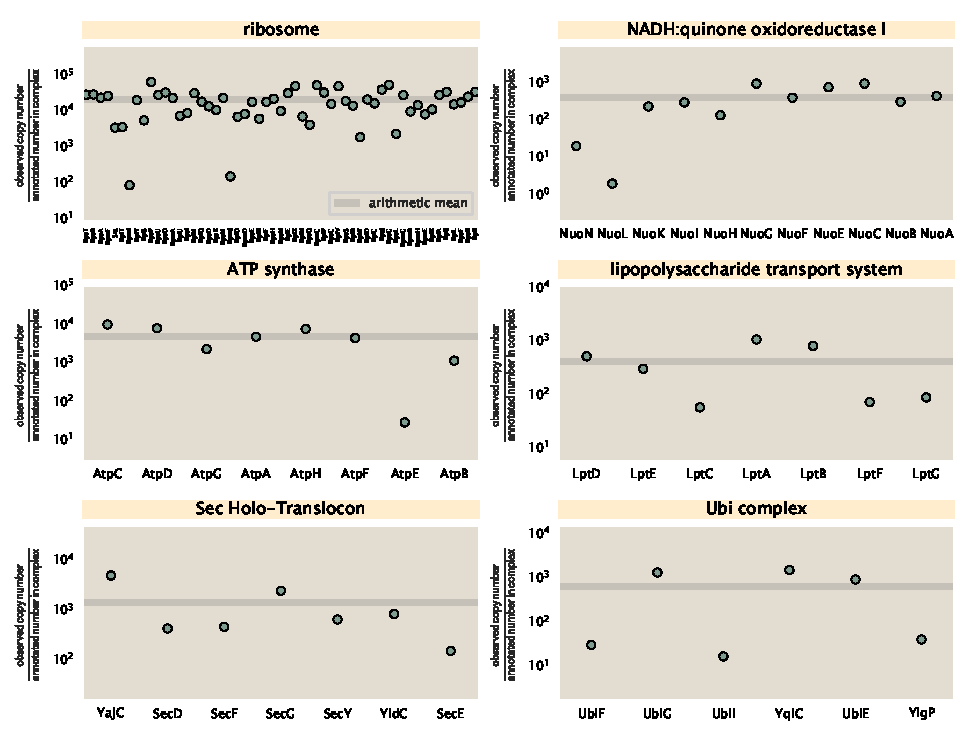
\includegraphics{SI_figs/figSX_subunit_counting.pdf}
            \caption{\textbf{Calculation of the mean complex abundance from
            measurements of single subunits.} Six of the largest complexes (by
            number of subunits) in \textit{E. coli}. Points correspond to the
            maximum number of complexes that can be formed given measurement of
            that individual protein. Solid grey line corresponds to the
            arithmetic mean across all subunits. These data correspond to
            measurements from \cite{schmidt2016} in a glucose-supplemented
            minimal growth medium.}
            \label{fig:complex_counting}
        }
    \end{fullwidth}
\end{figure}
